\chapter{Metamodel dla języka CAL}\label{chapter:cal-metamodel}

Aby otrzymać graficzny edytor modeli wykorzystując \SiriusWeb{} należy
najpierw zaprojektować metamodel danego języka w formacie \Ecore{}. Będzie on
opisywał strukturę modeli (składnię abstrakcyjną) oraz ich
reprezentację graficzną (składnię konkretną), która później będzie możliwa do
modyfikacji przez użytkowników. W tym rozdziale
zostanie omówiony język \emph{\acrfull{CAL}} służący do opisu obliczeń w
systemie \BalticLSC{}, a~następnie omówiony zostanie przygotowany w formacie
\Ecore{} metamodel.

\section{Język opisu obliczeń w BalticLSC}

Obliczenia rozproszone wykonywane przez system \BalticLSC{} są zapisywane w
formie \emph{aplikacji obliczeniowej}
(\emph{\selectlanguage{english}computation application})
korzystając ze składni języka \emph{\acrfull{CAL}} przygotowanego dla tego
właśnie systemu.

Podstawowym obiektem, który wysyła (wyjście)
lub odbiera (wejście) dane, jest \emph{pin}. Jest on~reprezentowany za pomocą
ikony kwadratu ze strzałką skierowaną w prawą stronę. Aplikacja obliczeniowa
składa się z wywołań jednostek obliczeniowych posiadających swoje piny, pinów
samej aplikacji obliczeniowej, oraz połączeń między tymi pinami. Grot
połączenia wskazuje kierunek przepływu danych.
Piny aplikacji obliczeniowej są zaznaczone na
diagramie ikoną pinu (strzałką skierowaną w prawo) z pogrubioną
jedną z krawędzi ikony --- lewą dla wejścia, prawą dla~wyjścia.

Jednostki obliczeniowe, które mogą być wywoływane przez aplikacje obliczeniową,
mogą być modułami obliczeniowymi napisanymi w wybranym języku programowania,
lub innymi aplikacjami obliczeniowymi, które z kolei mogą w swoim wnętrzu
wywoływać inne jednostki obliczeniowe. W ten sposób otrzymujemy możliwość
wykorzystania podzielenia skomplikowanej aplikacji obliczeniowej na mniejsze
części i wykorzystania ich, co pomaga w obniżeniu poziomu detali na jednym
diagramie i sprawia, że jest on łatwiejszy w zrozumieniu i modyfikacji.

Piny modułów oraz aplikacji obliczeniowych mają różne ikony, które
są ustalane na~podstawie ich właściwości. Są dwa kryteria wpływające na ikonę:

\begin{itemize}
	\item krotność danych, które obsługuje pin (\emph{data
		      multiplicity}):  dla pojedynczego pliku będzie
	      to~pojedyncza strzałka, a dla katalogu --- wiele strzałek,
	\item liczba pakietów przyjmowanych lub wysyłanych danych (\emph{token
		      multiplicity}, czy oczekuje pojedynczego zestawu danych
	      wejściowych, czy jednostka obsłuży kolejne zestawy danych
	      wysyłane po chwili
	      bez ponownego uruchomienia).
\end{itemize}

Moduł obliczeniowy rozpoczyna obliczenia dopiero gdy na każdym jego wejściu
znajdują się~dane.

Przykładowe aplikacje obliczeniowe zostały przedstawione na
rysunkach~\ref{rys:sekwencyjna-aplikacja-obliczeniowa}
i~\ref{rys:mozliwa-do-zrownoleglenia-aplikacja-obliczeniowa}.
Pierwsza z nich (rysunek~\ref{rys:sekwencyjna-aplikacja-obliczeniowa}) jest
aplikacją, w której obliczenia mogą zostać wykonane
wyłącznie sekwencyjnie, ponieważ dane przepływają sekwencyjnie od wejścia
kolejno przez jednostki nazwane \texttt{VideoToFrames}, \texttt{Face Detector},
\texttt{Blur Module}, \texttt{Blur module}, aż w końcu trafiają do wyjścia.
Inna jest struktura aplikacji na
rysunku~\ref{rys:mozliwa-do-zrownoleglenia-aplikacja-obliczeniowa}. Tam
przepływ danych rozdziela się~po~jednostce obliczeniowej \texttt{Pdf page
	splitter} i obliczenie jednostek \texttt{OCT Tesseract Tess 0.1} oraz
\texttt{OCR Tesseract LSTM 0.1} może zostać wykonane równolegle, być może
przez różne węzły obliczeniowe. Ich wyniki trafią później do jednostki
\texttt{Pdf data joiner 0.1} i~przejdą dalej przez pozostałe jednostki w sposób
sekwencyjny.

% \begin{noindent}
\begin{figure}[!hb]
	\centering

	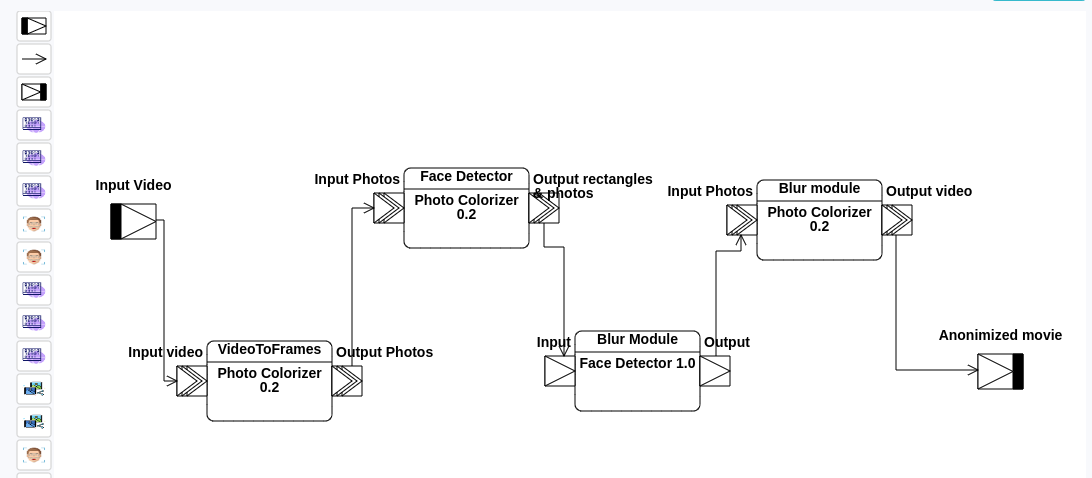
\includegraphics[width=0.95\linewidth]{./images/balticlsc-example-diagram.png}
	\caption{Aplikacja obliczeniowa w \BalticLSC{} z obliczeniami
		sekwencyjnymi}\label{rys:sekwencyjna-aplikacja-obliczeniowa}
	\medskip
	{\small Źródło: aplikacja obliczeniowa \emph{Pdf to readable pdf converter} z
		systemu \emph{BalticLSC},\\
    % NOTE: to nie może być \footnote, Latex wyrzuca wtedy błąd
		\url{https://balticlsc.iem.pw.edu.pl/#/computation-application/5532b8b8-a39c-4725-8880-80ec5b2207a4}
  }
\end{figure}
% \end{noindent}

% \begin{noindent}
\begin{figure}[!ht]
	\centering

	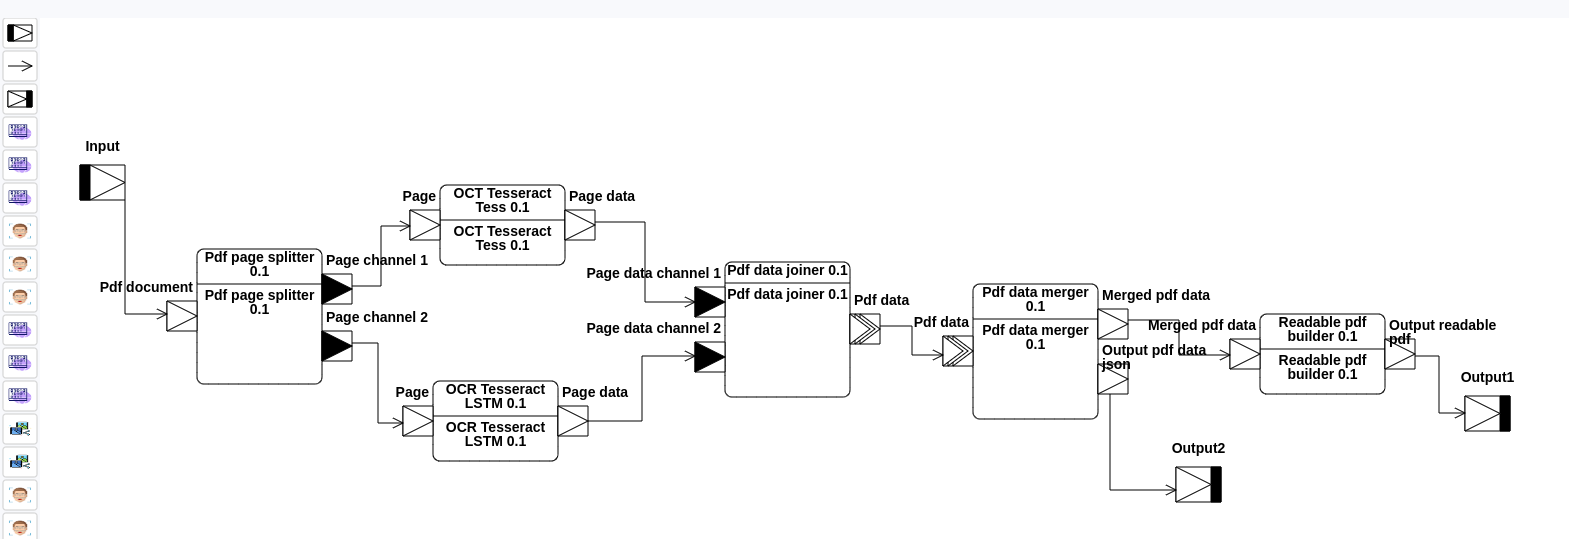
\includegraphics[width=0.99\linewidth]{./images/balticlsc-concurrent-application-example.png}
	\caption{Aplikacja obliczeniowa w \BalticLSC{} z możliwością
		zrównoleglenia obliczeń}\label{rys:mozliwa-do-zrownoleglenia-aplikacja-obliczeniowa}
  \medskip
  {\small Źródło: aplikacja obliczeniowa \emph{Movie test}
    z systemu \emph{BalticLSC},\\
    \url{https://balticlsc.iem.pw.edu.pl/#/computation-application/27571955-6e2b-4735-85ea-44f5438ca7f6}}
\end{figure}
% \end{noindent}

\section{Zaprojektowany metamodel dla języka CAL}

Składnia abstrakcyjna przygotowanego w formacie \Ecore{} metamodelu dla języka
\CAL{} widoczna jest na
rysunku~\ref{rys:cal-emf-metamodel}. Jego składnia konkretna
jest omówiona w dalszej części pracy i będzie przedstawiona na
rysunku~\ref{rys:sirius-desktop-cal-example-model}.
Przygotowany metamodel bazuje na metamodelu
opracowanym w ramach projektu \BalticLSC{}~\cite{cal-metamodel}, którego
składnia abstrakcyjnna jest widoczna
na~rysunku~\ref{rys:cal-metamodel-balticlsc}.
Na potrzeby edytora diagramów nie są potrzebne wszystkie elementy oryginalnego
metamodelu. Niektóre klasy i~właściwości zostały pominięte, ponieważ nie były
istotne z~perspektywy edycji diagramu.
W przygotowanym metamodelu niektóre klasy są nowe, lub pomimo podobnej nazwy
mają inne znaczenie od tych w metamodelu języka \CAL{} z systemu \BalticLSC{}.
Taki zabieg został wykonany aby uprościć metamodel, ponieważ jego przeznaczenie
jest inne (wyłącznie edycja diagramów aplikacji obliczeniowych) w porównaniu z
metamodelem z systemu \BalticLSC{} (wykonywanie obliczeń zgodnie z modelem).
Różnice zostaną opisane w~dalszej części pracy.

\begin{figure}[!ht]
	\centering

	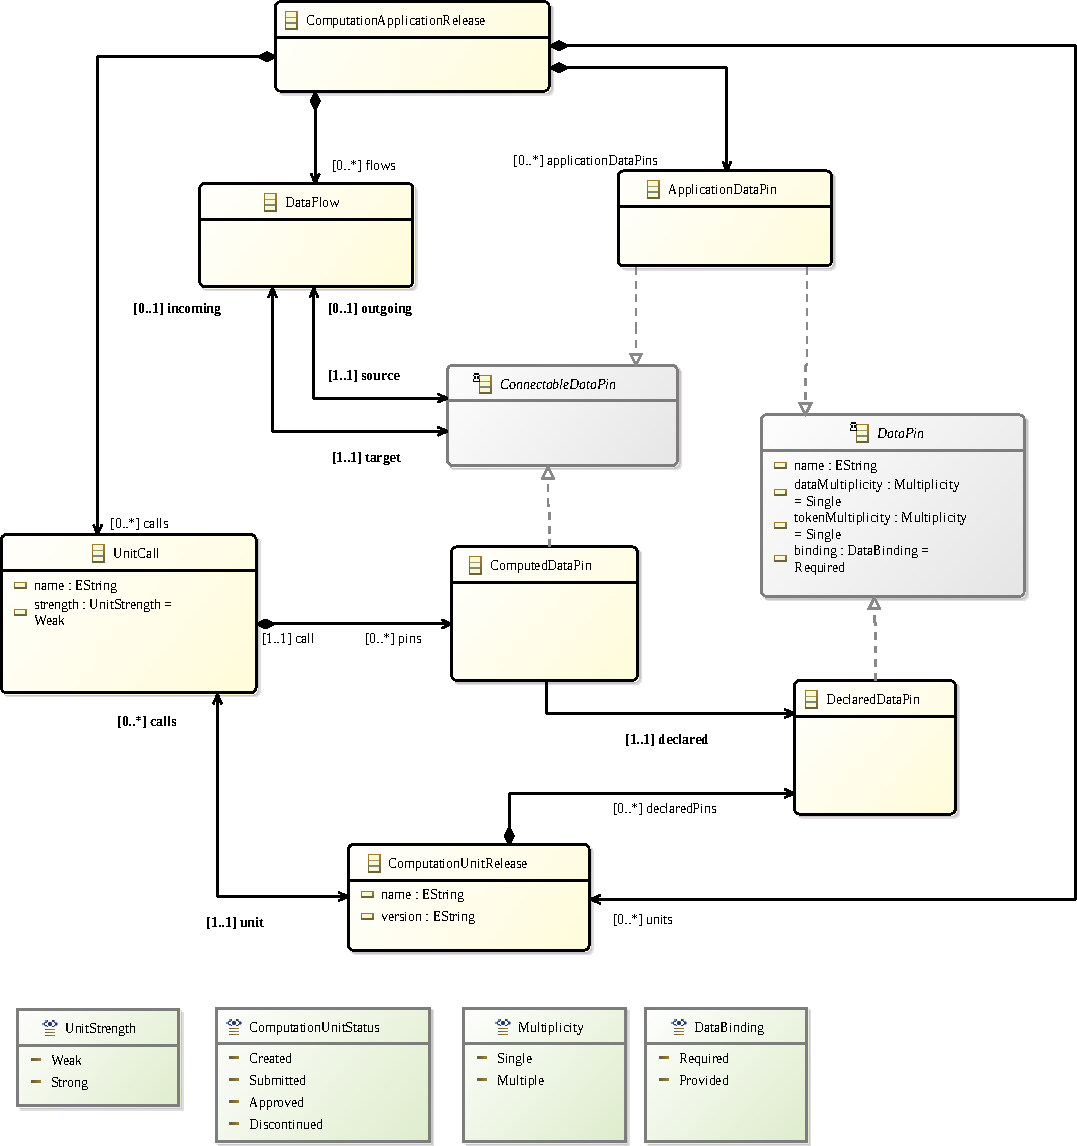
\includegraphics[width=0.92\linewidth]{./images/cal-emf-metamodel.pdf}
	\caption{Metamodel w formacie \Ecore{} dla języka \CAL{} przygotowany w
		ramach tej pracy}\label{rys:cal-emf-metamodel}
\end{figure}

Model bazujący na metamodelu w formacie \Ecore{} ma strukturę grafową. Głównym
jego elementem jest obiekt typu
\texttt{Computation\-Application\-Release}, który odpowiada całemu diagramowi
(aplikacji obliczeniowej). Nie~ma~on~własnych właściwości. Zawiera on w sobie
natomiast 4 typy obiektów:

% NOTE: placing this figure before the list makes it break the list, which is
% expected
% \begin{noindent}
\begin{figure}[!hb]
	\centering

	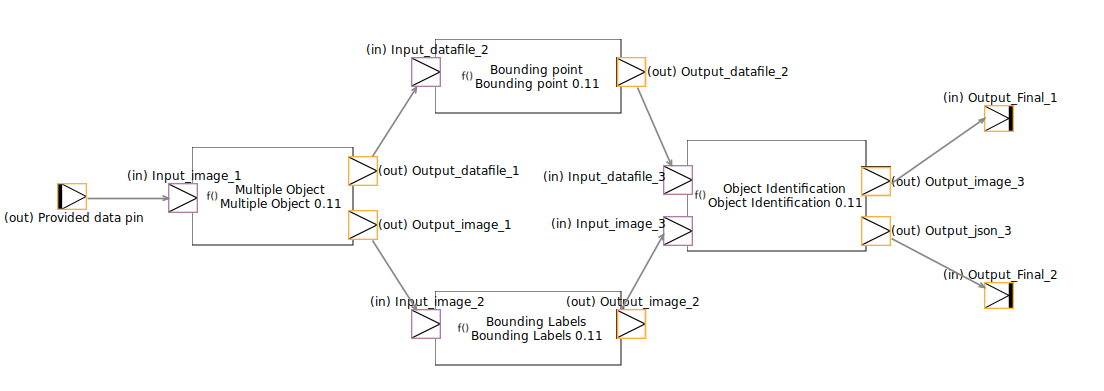
\includegraphics[width=0.99\linewidth]{./images/sirius-desktop-cal-example-model.png}
	\caption{Składnia konkretna przygotowanego metamodelu języka \CAL{} w
		\SiriusDesktop{}}\label{rys:sirius-desktop-cal-example-model}
\end{figure}
% \end{noindent}

\begin{itemize}
	\item \texttt{ComputationUnitRelease} --- są to obiekty odpowiadające
	      rodzajom modułów i~aplikacji obliczeniowych dostępnych w systemie
	      \BalticLSC{} i opisują ich właściwości.

	      Oprócz informacji o nazwie i wersji jednostki obliczeniowej
	      zawierają w sobie obiekty \texttt{DeclaredDataPin} dziedziczące z
	      \texttt{DataPin}, które opisują piny tej jednostki obliczeniowej.

	      W przygotowanym metamodelu dla języka \CAL{} obiekty typu
	      \texttt{Computation\-Unit\-Release} reprezentują zarówno moduły
	      obliczeniowe,
	      jak i aplikacje obliczeniowe, które w~oryginalnym metamodelu z
	      systemu
	      \BalticLSC{} są dwoma osobnymi rodzajami obiektów. Z perspektywy
	      edytora
	      diagramów nie ma znaczenia czy wywoływana jednostka obliczeniowa
	      jest modułem
	      obliczeniowym, czy aplikacją obliczeniową składającą
	      się~z~wywołań innych
	      jednostek obliczeniowych. Uproszczenia tego dokonano aby uniknąć
	      umieszczania w
	      modelu zbyt szczegółowych i niepotrzebnych informacji.

	      Obiekty te nie są wyświetlane na diagramie (nie występują w
	      wizualnej reprezentacji modelu). Można je zobaczyć jedynie w
	      drzewie obiektów
	      modelu.

	\item \texttt{UnitCall} --- wywołania dostępnych jednostek
	      obliczeniowych. Każda dostępna jednostka obliczeniowa może zostać
	      wywołana dowolną liczbę razy. Każde wywołanie to~osobny obiekt
	      \texttt{UnitCall} ze wskazaniem jednostki, która ma zostać
	      wywołana, a~także
	      z~obiektami \texttt{ComputedDataPin}, które reprezentują piny tej
	      jednostki.

	      Taka reprezentacja pozwala na zapisanie szczegółów dotyczących
	      dostępnych jednostek obliczeniowych wyłącznie raz w modelu, a
	      później
	      wskazywanie tych elementów w~każdym z wywołań jednostki.

	      Rozwiązanie to ma jednak pewne ograniczenie --- aby oznaczyć
	      wywołanie jednostki za~pomocą obiektu \texttt{UnitCall}, należy
	      najpierw
	      stworzyć obiekt \texttt{Computation\-Unit\-Release} i~dodać
	      odpowiednie
	      \texttt{Declared\-Data\-Pin}. Można wywołać jedynie jednostki,
	      które
	      są~zapisane w metamodelu. Edytor modeli domyślnie nie ma
	      możliwości pobrania
	      informacji o~dostępnych jednostkach obliczeniowych z systemu
	      \BalticLSC{}, więc
	      to~użytkownik musi samemu dodać dostępne jednostki do metamodelu.

	      Na diagramie obiekty te są reprezentowane jako prostokąty ze
	      swoimi pinami umieszczonymi na krawędziach. Wewnątrz prostokąta
	      znajduje się
	      etykieta zawierająca nazwę umożliwiającą wyróżnienie tego
	      konkretnego wywołania
	      jednostki, oraz nazwę i wersję wydania wywoływanej jednostki.
	      Składnię
	      konkretną widać na
	      rysunku~\ref{rys:sirius-desktop-cal-example-model}.
	      Piny~wywołania jednostek obliczeniowych
	      (\texttt{ComputedDataPin}) są również
	      na nim widoczne jako prostokąty z ikoną strzałki w prawo.

	\item \texttt{ApplicationDataPin} --- piny aplikacji obliczeniowej
	      opisywanej przez ten model. Są~to~wejścia i wyjścia z diagramu.
	      Właściwości pinu są dziedziczone z klasy \texttt{DataPin}. Z
	      uwagi na fakt, że
	      te piny będą łączone z innymi pinami, klasa ta dziedziczy z klasy
	      \texttt{ConnectableDataPin}.

	      Na diagramie obiekty te reprezentowane są jako prostokąty z ikoną
	      strzałki w prawo z~pogrubionym prawym lub lewym jej bokiem, co
	      widać na
	      rysunku~\ref{rys:sirius-desktop-cal-example-model}.

	      W metamodelu języka \CAL{} z systemu \BalticLSC{} te obiekty są
	      reprezentowane za~pomocą klasy \texttt{DeclaredDataPin}, która w
	      metamodelu
	      tworzonym na potrzeby edytora jest inną klasą. Powodem tego był
	      fakt, że z
	      perspektywy aktualnie edytowanej aplikacji obliczeniowej, jej
	      piny są logicznie
	      innym bytem niż piny wywoływanych przez nią jednostek
	      obliczeniowych.
	      \texttt{ApplicationDataPin} powinny być połączone z innymi
	      pinami w modelu, podczas gdy \texttt{DeclaredDataPin} są jedynie
	      definicjami pinów i nie powinny mieć wychodzących lub wchodzących
	      połączeń.
	      Mają też
	      inną składnię konkretną (\texttt{DeclaredDataPin}
	      nie~są~wyświetlane na
	      diagramie, a piny aktualnie edytowanej aplikacji obliczeniowej
	      są).

	\item \texttt{DataFlow} --- połączenia między pinami
	      (\texttt{ConnectableDataPin}) umieszczonymi na~wywołaniach
	      jednostek obliczeniowych (\texttt{ComputedDataPin} na
	      \texttt{UnitCall}) lub pinami aktualnie opisywanej aplikacji
	      obliczeniowej
	      (\texttt{ApplicationDataPin}).

	      Na diagramie obiekty te reprezentowane są jako krawędzie z grotem
	      wskazującym kierunek przepływu danych, co widać na
	      rysunku~\ref{rys:sirius-desktop-cal-example-model}.
\end{itemize}

Składnia konkretna przygotowanego metamodelu języka \CAL{} wyświetlona w
programie \SiriusDesktop{} dla przykładowego modelu została przedstawiona na
rysunku~\ref{rys:sirius-desktop-cal-example-model}.

Oprócz podstawowej struktury metamodelu oraz jego reprezentacji w formie
diagramu zostały do niego dodane dodatkowe funkcjonalności dostępne w ramach
technologii \EMF{}. Zostały one opisane
w kolejnych sekcjach.

Składnia abstrakcyjna metamodelu języka \CAL{} używanego w systemie
\BalticLSC{}, na~którym wzorowano metamodel przygotowany w ramach tej pracy
magisterskiej, widoczna jest na~rysunku~\ref{rys:cal-metamodel-balticlsc}.

\begin{figure}[!ht]
	\centering

	% NOTE: this image is pretty tall, so it must be kept much smaller than the
	% line width so it does not take up the whole page, moving all incoming
	% images to the bottom of the chapter.

	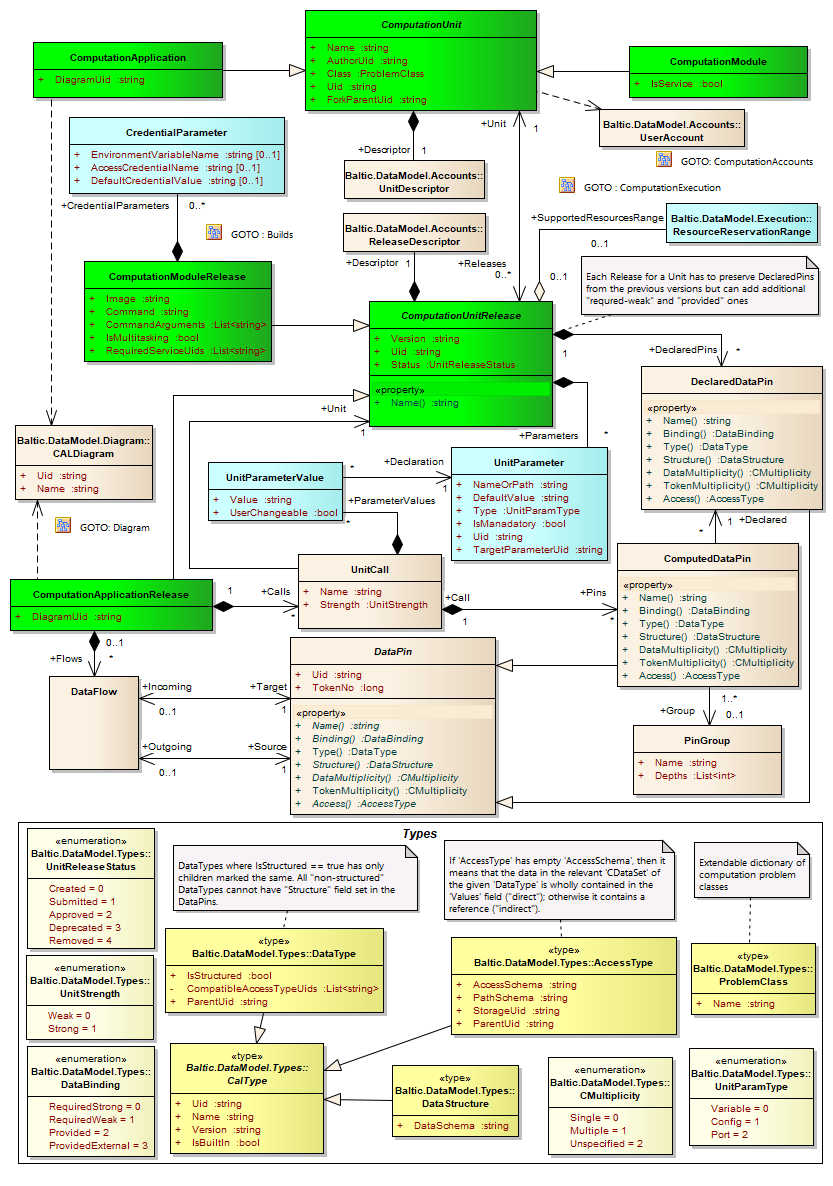
\includegraphics[width=0.82\linewidth]{./images/cal-metamodel-balticlsc.png}
	\caption{Składnia abstrakcyjna metamodelu języka \CAL{} używanego w
		projekcie \BalticLSC{}}\label{rys:cal-metamodel-balticlsc}

	\medskip
	{\small Źródło:
		\url{https://www.balticlsc.eu/model/index.htm?goto=4:2:404}}
\end{figure}

\subsection{Warunkowa zmiana stylu elementów}

% \begin{noindent}
Użytkownik może wywnioskować dodatkowe informacje z diagramu jeżeli jego wygląd
będzie zależał od właściwości elementów modelu. Takie rozwiązanie zastosowano
dla dwóch elementów metamodelu dzięki wykorzystaniu \emph{Style
	Customizations}~\cite{sirius-desktop-documentation-style-customizations}
z technologii \EMF{}.
% \end{noindent}
Funkcjonalność ta pozwala na wskazanie za pomocą języka \AQL{} w jakich
sytuacjach styl elementu powinien zostać zmieniony, a następnie wskazać które
właściwości powinny ulec zmianie oraz ich nowe wartości.

Pierwszy styl warunkowy został użyty dla pinów w metamodelu. Piny
(\texttt{DataPin}) zmieniają ikonę na podstawie swoich krotności danych oraz
paczek danych (odpowiednio \emph{data multiplicity} i \emph{token
	multiplicity}).

Z uwagi na fakt, że oba parametry mogą mieć jedną z 2 wartości,
co daje w sumie 4~możliwości, w klasie \texttt{Services} metamodelu stworzono
metodę w języku \Java{}, która zwraca nazwę odpowiedniej ikony.
Dzięki możliwości wykorzystania języka programowania osiągnięto
zamierzony efekt za pomocą jednego stylu warunkowego, a nie 4 różnych
styli dla 4 możliwości. Kod metody zwracającej nazwę ikony dla pinu
został przedstawiony w listingu~\ref{lst:getDataPinIconPath-method}.

\begin{lstlisting}[float,
    floatplacement=ht,
    language=Java,
    caption={Metoda zwracająca nazwę ikony dla pinu},
    label={lst:getDataPinIconPath-method}]
public String getDataPinIconPath(EObject self) {
  if (!(self instanceof DataPin)) {
    return null;
  }

  var dataPin = (DataPin) self;
  var dataPart = dataPin.getDataMultiplicity() == Multiplicity.SINGLE ? "single-data" : "multiple-data";
  var tokenPart = dataPin.getTokenMultiplicity() == Multiplicity.SINGLE ? "single-token" : "multiple-tokens";

  return dataPart + "-" + tokenPart + ".png";
}
\end{lstlisting}

Dla pinów całej aplikacji obliczeniowej (\texttt{Application\-Data\-Pin} dla
\texttt{Computation\-Application\-Release}) styl warunkowy był
rozszerzeniem tego
dla pinów wywoływanych jednostek obliczeniowych. Oprócz brania pod uwagę
krotności danych
oraz
paczek danych, w~tym~stylu znaczenie ma ponadto kierunek pinu. Piny wejściowe
mają pogrubiony pasek z~lewej strony, a~piny wyjściowe z prawej. Dla tych
pinów występują 3 cechy od których zależy ikona, co oznacza 8 możliwości.
Dzięki wykorzystaniu metody z listingu~\ref{lst:getDataPinIconPath-method} oraz
języka \AQL{} ta~funkcjonalność została zrealizowana za pomocą jednego stylu
warunkowego, zamiast 8~styli dla 8 różnych wariantów.

Drugim wykorzystanym rodzajem styli warunkowych jest zmiana koloru obramowania
pinów na krawędziach wywoływanych jednostek obliczeniowych
(\texttt{ComputedDataPin}) w
zależności od~kierunku przepływu danych. Piny wejściowe (\emph{required}) mają
ramkę koloru fioletowego, a~piny wyjściowe (\emph{provided}) mają ramkę koloru
pomarańczowego. Ta funkcjonalność została zaimplementowana za pomocą jednego
stylu warunkowego.

Wyniki działania obu rodzajów styli warunkowych widoczne są na
rysunku~\ref{rys:sirius-desktop-cal-example-model} pokazującym
składnię konkretną metamodelu.

\subsection{Narzędzia edytora diagramów}\label{sec:cal-metamodel-tools}

Dla metamodeli w formacie \Ecore{} można zdefiniować narzędzia wspomagające i
ułatwiające edycję modeli, a także pomagające uniknąć
błędów semantycznych~\cite{sirius-desktop-documentation-tools}. Również do
metamodelu języka
\CAL{} dodano takie narzędzia, które zostaną omówione w tej sekcji.

Pierwszą grupą narzędzi dodanych do przygotowanego metamodelu języka \CAL{} są
narzędzia
automatyzujące pracę użytkownika, aby ten nie musiał manualnie wykonywać
niektórych czynności, a~jednocześnie aby w modelu nie znajdowały się nieużywane
elementy.

Jednym z takich narzędzi jest automatyczne usuwanie połączeń między pinami
w~momencie, gdy ten pin zostaje usunięty. W przypadku pinów aplikacji
obliczeniowej (\texttt{Application\-Data\-Pin}) narzędzie to zastępuje zwykłą
operację usunięcia. Dla pinów wywołania jednostki obliczeniowej
(\texttt{ComputedDataPin}), narzędzie to uruchamiane jest podczas usuwania
tej~jednostki obliczeniowej. Dzięki temu narzędziu w modelu nie pozostają
połączenia
zakończone jedynie z jednej strony.

Drugim z narzędzi automatyzujących pracę jest automatyczne zarządzanie
pinami wywołania jednostki obliczeniowej (\texttt{ComputedDataPin}) w~momencie
wskazania lub zmiany która jednostka obliczeniowa ma zostać wywołana. Zmiana
atrybutu \texttt{unit} obiektu \texttt{UnitCall} usuwa aktualnie powiązane z
nim piny (o ile jakieś istniały) i tworzy nowe na podstawie definicji jednostki
obliczeniowej (\texttt{ComputationUnitRelease}) zapisanej w metamodelu,
a~także jej~zdeklarowanych pinów (\texttt{DeclaredDataPin}). Stworzone piny
mają
automatycznie ustawione odwołania na właściwe deklaracje pinów.
Wykorzystanie tego narzędzia zostało przedstawione na
rysunku~\ref{rys:sirius-desktop-change-unit-to-call}.
Rysunek~\ref{rys:sirius-desktop-empty-unit-call} demonstruje wygląd nowo
utworzonego wywołania jednostki obliczeniowej bez wskazania którą jednostkę ono
wywołuje. Po wskazaniu jednostki do~wywołania, piny są tworzone automatycznie,
co
widać na rysunku~\ref{rys:sirius-desktop-change-unit-to-call-before}. Po
ponownej zmianie jednostki obliczeniowej do wywołania, poprzednie piny są
usuwane, a na ich miejsce zostają utworzone nowe, na bazie definicji wybranej
jednostki obliczeniowej, co widać na
rysunku~\ref{rys:sirius-desktop-change-unit-to-call-after}.

% \begin{noindent}
\begin{figure}[h]
	\centering
	\begin{subfigure}{.3\textwidth}
		\centering
		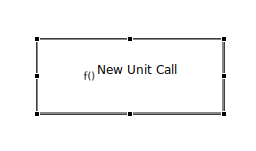
\includegraphics[width=.99\linewidth]{./images/sirius-desktop-empty-unit-call.png}
		\caption{Nowo utworzone wywołanie jednostki obliczeniowej}\label{rys:sirius-desktop-empty-unit-call}
	\end{subfigure}
	\begin{subfigure}{.3\textwidth}
		\centering
		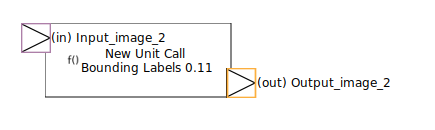
\includegraphics[width=.99\linewidth]{./images/sirius-desktop-change-unit-to-call-before.png}
		\caption{Wywołanie jednostki obliczeniowej po wskazaniu jednostki do
      wywołania}\label{rys:sirius-desktop-change-unit-to-call-before}
	\end{subfigure}
	\begin{subfigure}{.3\textwidth}
		\centering
		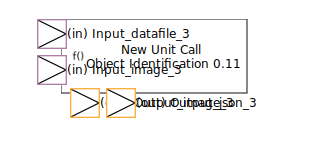
\includegraphics[width=.99\linewidth]{./images/sirius-desktop-change-unit-to-call-after.png}
		\caption{Wywołanie jednostki obliczeniowej po ponownym wskazaniu jednostki do
        wywołania}\label{rys:sirius-desktop-change-unit-to-call-after}
	\end{subfigure}

	\caption{Demonstracja działania narzędzia zarządzającego pinami wywołań
    jednostek obliczeniowych}\label{rys:sirius-desktop-change-unit-to-call}
\end{figure}
% \end{noindent}

Narzędzie to zostało przygotowane poprzez modyfikację kodu źródłowego klas
metamodelu. Została zmieniona definicja metody zmiany wskazania na jednostkę do
wywołania w obiekcie \texttt{UnitCall}. Podczas wywołania tej metody usuwane są
poprzednie piny i tworzone są nowe. To zachowanie opisane jest w języku
\Java{}.

Dzięki temu narzędziu użytkownik nie musi samemu usuwać starych pinów
i~tworzyć nowych podczas zmiany wywoływanej jednostki obliczeniowej.
Przyśpiesza to~pracę z
metamodelem i~pomaga uniknąć błędów.

Inną grupą narzędzi są narzędzia pomagające w przestrzeganiu poprawności
modelu. Do~tej~grupy można zaliczyć kilka narzędzi dotyczących tworzenia lub
modyfikacji połączeń między pinami. Dane mogą przepływać jedynie od pinów
wyjściowych do pinów wejściowych. Ponadto, niemożliwe jest połączenie pinów
na tym samym wywołaniu jednostki obliczeniowej. Oba te wymagania mogą być
egzekwowane w modelu za pomocą narzędzi do~tworzenia połączeń (\emph{Edge
	Creation}) oraz do zmiany połączenia (\emph{Reconnect Edge}). Pierwsze
z nich za~pomocą warunków \emph{Connection Start Precondition} oraz
\emph{Connection Complete Precondition}, ustalających czy połączenie może
zostać
rozpoczęte lub zakończone w~danym elemencie, pozwala zabronić stworzenia
połączenia. Drugie z nich za pomocą warunku \emph{Precondition} ustala kiedy
zmiana jednego z końców połączenia jest możliwa.

Drugim z narzędzi w grupie pomagających w przestrzeganiu poprawności jest
narzędzie uniemożliwiające usuwanie pinów wywołań jednostek obliczeniowych
(\texttt{ComputedDataPin}). Są one tworzone i usuwane automatycznie podczas
wskazania jednostki do wywołania i~niepoprawnym byłoby gdyby użytkownik mógł
tworzyć lub usuwać je samemu, ponieważ faktyczna liczba pinów mogłaby się
wtedy nie
zgadzać z liczbą zadeklarowanych pinów w~tej~jednostce obliczeniowej.

Innym typem narzędzi są narzędzia ułatwiające tworzenie elementów modelu.
Są~3~proste narzędzia umieszczających element w modelu: dla pinu wejściowego i
wyjściowego aplikacji, a także dla pustego wywołania jednostki obliczeniowej,
dla
którego należy później wskazać jednostkę, którą ma wywołać. Bardziej
skomplikowanym
narzędziem jest narzędzie pozwalające na~dodanie do modelu wywołania jednostki
obliczeniowej, które pokazuje okno dialogowe pozwalające wybrać jednostkę oraz
wskazać nazwę dodawanego obiektu. Wykorzystuje ono~możliwości \SiriusDesktop{}
do tworzenia okien dialogowych (zarówno jednorazowych
jak~i~składających się z wielu
kroków)~\cite{sirius-desktop-documentation-tools} i
pozwala na dostarczeniu użytkownikowi
bardziej interaktywnych i przyjemniejszych wrażeń z pracy z modelem. Okno
dialogowe
pokazujące się po wybraniu
tego narzędzia jest przedstawione na
rysunku~\ref{rys:sirius-desktop-create-unit-call-tool}.

% \begin{noindent}
\begin{figure}[!hb]
	\centering

	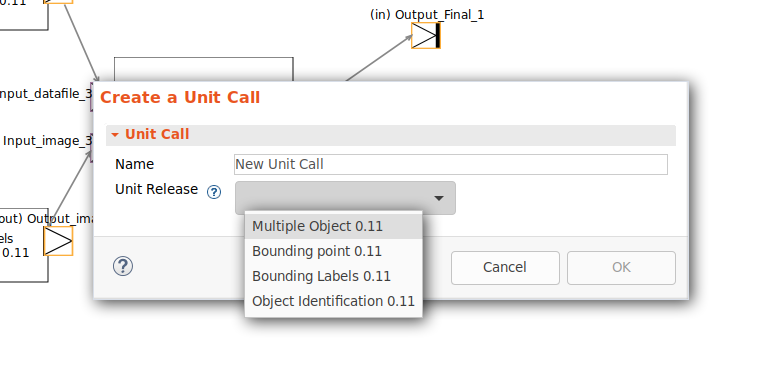
\includegraphics[width=0.95\linewidth]{./images/sirius-desktop-create-unit-call-tool.png}
	\caption{Narzędzie do interaktywnego tworzenia nowego wywołania jednostki
		obliczeniowej w~\SiriusDesktop{}}\label{rys:sirius-desktop-create-unit-call-tool}
\end{figure}
% \end{noindent}

Narzędzia te uruchamiają się jedynie, gdy zmiana w modelu zostanie wykonana
poprzez edycję diagramu lub właściwości już istniejącego elementu. Podczas
bezpośredniej edycji drzewa modelu narzędzia powiązane z metamodelem są
pomijane, przez co można doprowadzić do~sytuacji, w której model nie będzie
poprawny
semantycznie. Przykładem operacji pomijającej narzędzia jest usunięcie pinu
aplikacji obliczeniowej (\texttt{ApplicationDataPin}) bezpośrednio z~drzewa
modelu. Jeżeli miała ona połączenie (\texttt{DataFlow}), nie zostanie
ono~automatycznie usunięte (narzędzie, które je usuwa nie zostanie
uruchomione), co
prowadzi do istnienia w~modelu połączenia, którego jedynie jeden koniec jest
poprawnie ustawiony. Takie sytuacje natomiast są wykrywane przez reguły
walidacji strukturalnej metamodelu (połączenie musi mieć poprawne oba końce).

\subsection{Reguły walidacyjne powiązane z
	metamodelem}\label{sec:reguly-walidacyjne-metamodel}

\SiriusDesktop{} dostarcza mechanizm walidacji edytowanego modelu. Można
go uruchomić poprzez wybranie opcji \menu{Diagram > Validate} z głównego menu
programu. Wyświetlona zostanie wtedy lista informacji diagnostycznych
dotyczących modelu.

\SiriusDesktop{} domyślnie dostarcza informacji o błędach składniowych
modelu. Będą to~ostrzeżenia o braku wymaganych atrybutów lub niepoprawnej
krotności elementów (jeżeli dana właściwość powinna zawierać przykładowo co
najmniej 3 elementy, a nie więcej niż~5~elementów). Błędy te będą także
zaznaczone na diagramie za pomocą ikony czerwonego znaku \texttt{X} obok
elementu, którego wiadomość dotyczy. Zostało to zilustrowane na
rysunku~\ref{rys:sirius-desktop-syntax-validation}.
Ostatni wiersz na liście problemów jest związany z walidacją składniową i
wskazuje on, że~obiekt odpowiadający wywołaniu jednostki obliczeniowej nie ma
ustawionego atrybutu \texttt{unit}, czyli brakuje wskazania jednostki do
wywołania. Ta sama wiadomość jest widoczna na diagramie po przeniesieniu
kursora na znak \texttt{X}.
Reszta problemów na liście wynika z błędów edytora, a~nie~modelu, więc została
rozmyta dla zwrócenia uwagi na informacje pochodzące z walidacji składniowej.

% \begin{noindent}
\begin{figure}[!hb]
	\centering

	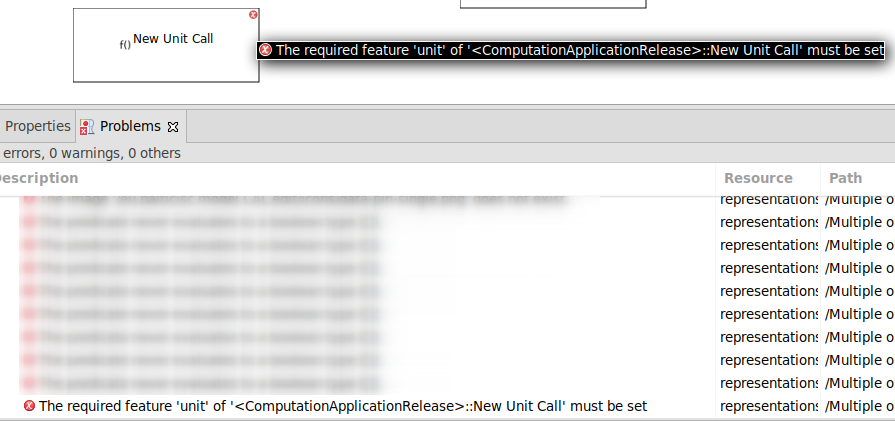
\includegraphics[width=0.95\linewidth]{./images/sirius-desktop-syntax-validation.png}
	\caption{Walidacja składniowa modeli w \SiriusDesktop{}}\label{rys:sirius-desktop-syntax-validation}
\end{figure}
% \end{noindent}

Dodatkowo w pliku \texttt{*.odesign} pakietu \texttt{.design} metamodelu można
zdefiniować \emph{Semantic Validation
	Rules}~\cite{sirius-desktop-documentation-validation-rules}.
Pozwalają one na dodanie własnych reguł walidacji semantycznej modeli. To
reguły powinny opisywać ograniczenia, których nie dostarcza opis struktury
modelu i~zależą od połączenia kilku elementów ze sobą. Można
wybrać jakich elementów reguła dotyczy, a~za~pomocą języka \AQL{} wskazać
kiedy informacja diagnostyczna powinna być pokazana, a także jaka powinna być
wiadomość wyświetlona użytkownikowi, oraz z jakim poziomem poważności
(informacja, ostrzeżenie, błąd). Jeżeli wiadomo jak można naprawić błąd, można
zdefiniować również sekwencję akcji, które będą wykonywane gdy użytkownik
wybierze
opcje automatycznego naprawiania błędów diagnostycznych.

Przykładową regułę walidacji semantycznej przedstawiono na
rysunku~\ref{rys:sirius-desktop-example-semantic-validation-rule}.
Zabrania ona~połączeń między pinami znajdującymi się na tym samym wywołaniu
jednostki obliczeniowej. Jej struktura wyrażona w drzewie obiektów metamodelu
jest widoczna na
rysunku~\ref{rys:sirius-desktop-example-semantic-validation-rule-tree},
a~jej~właściwości na
rysunku~\ref{rys:sirius-desktop-example-semantic-validation-rule-properties}.
Widać tam element, dla którego wiadomość zostanie wyświetlona
(\texttt{DataFlow}).
Rysunek~\ref{rys:sirius-desktop-example-semantic-validation-rule-audit}
przedstawia wyrażenie języka \AQL{}. Niespełnienie warunku spowoduje
pokazanie
informacji o błędzie. W tym przypadku sprawdza ono, czy~obiekty początkowy i
końcowy połączenia mają różnych rodziców. Nie jest to spełnione wyłącznie
jeżeli oba~piny należą do tego samego wywołania jednostki obliczeniowej.
Błąd wynikający z tej reguły został
przedstawiony na
rysunku~\ref{rys:sirius-desktop-example-semantic-validation-rule-failure}.
Należało wykluczyć sytuacje, w
których połączenie jest między dwoma pinami aplikacji obliczeniowej, ponieważ
takie połączenia są~dozwolone.

% \begin{noindent}
\begin{figure}[!ht]
	\centering
	\begin{subfigure}{.8\textwidth}
		\centering
		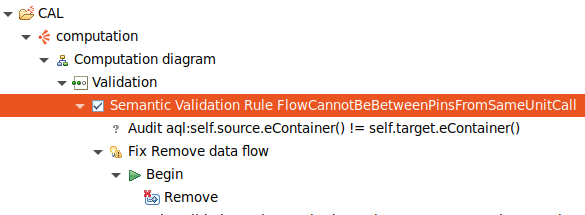
\includegraphics[width=.99\linewidth]{./images/sirius-desktop-example-semantic-validation-rule-tree.png}
		\caption{Drzewo obiektów składających się na regułę walidacji
      semantycznej}\label{rys:sirius-desktop-example-semantic-validation-rule-tree}
	\end{subfigure}

  \medskip

	\begin{subfigure}{.92\textwidth}
		\centering
		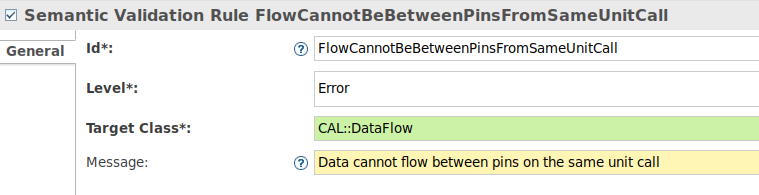
\includegraphics[width=.99\linewidth]{./images/sirius-desktop-example-semantic-validation-rule-properties.png}
		\caption{Właściwości reguły walidacji semantycznej}\label{rys:sirius-desktop-example-semantic-validation-rule-properties}
	\end{subfigure}

  \medskip

	\begin{subfigure}{.92\textwidth}
		\centering
		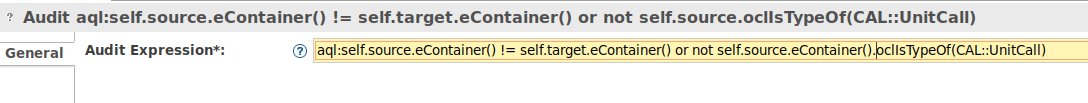
\includegraphics[width=.99\linewidth]{./images/sirius-desktop-example-semantic-validation-rule-audit.png}
		\caption{Warunek spełnienia reguły walidacji semantycznej}\label{rys:sirius-desktop-example-semantic-validation-rule-audit}
	\end{subfigure}

  \begin{subfigure}{.92\textwidth}
    \centering
    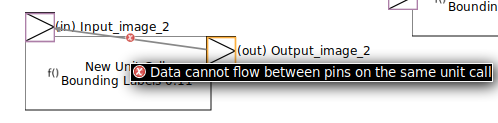
\includegraphics[width=.99\linewidth]{./images/sirius-desktop-example-semantic-validation-rule-failure.png}
    \caption{Błąd --- reguła nie została
    spełniona}\label{rys:sirius-desktop-example-semantic-validation-rule-failure}
  \end{subfigure}

	\caption{Przykładowa reguła walidacji semantycznej w \emph{Sirius
    Desktop}}\label{rys:sirius-desktop-example-semantic-validation-rule}
  \medskip
\end{figure}
% \end{noindent}

Oprócz reguły walidacji semantycznej zaprezentowanej na
rysunku~\ref{rys:sirius-desktop-example-semantic-validation-rule}
zaprojektowano 5~innych reguł informujących użytkownika o błędach w metamodelu.
Pierwsze dwie z~nich pomagają ustalić oczekiwany kierunek połączeń pinów. Dla
pinów oznaczonych jako wymagane (\texttt{required}) połączenie powinno być
wchodzące, a dla pinów oznaczonych jako dostarczone (\texttt{provided}) ---
wychodzące. Jest to informacja niewynikająca ze struktury metamodelu, więc
została dostarczona jako reguła walidacji semantycznej. Oprócz 2 reguł
wymagających połączenia danego typu są też 2 reguły, które zabraniają
połączenia w~przeciwną stronę niż~oczekiwana. Oznacza to, że jeżeli pin nie
będzie miał żadnego połączenia, będzie pokazana informacja o braku, a jeżeli
dodatkowo pin będzie miał połączenie w~przeciwną stronę (przykładowo, pin
wymagany będzie miał połączenie wychodzące), to będą 2~wiadomości: jedna o
braku połączenia w oczekiwanym kierunku, a druga o~nieoczkiewanym połączeniu
w~przeciwnym kierunku.

Ostatnią dodaną regułą jest sprawdzenie czy oba końce połączenia (obiektu
\texttt{DataFlow}) są~zdefiniowane. Jeżeli krawędź nie jest połączona z dwoma
obiektami, użytkownik dostaje o tym informacje oraz możliwość szybkiego
usunięcia takiego połączenia. Jest to szczególnie ważne, ponieważ takie
połączenia nie są pokazywane na diagramie, a jedynie wprowadzają zamieszanie w
metamodelu i utrudniają badanie jego struktury przez narzędzia, które muszą
oczekiwać, że krawędzie mogą nie być zaczepione z obu stron.

\subsection{Testy metamodelu}\label{sec:testy-metamodelu}

W sekcji~\ref{sec:cal-metamodel-tools} opisano modyfikacje kodu źródłowego klas
metamodelu, które usprawniają pracę użytkownika z modelem. Aby upewnić się, że
te modyfikacje działają poprawnie, należy je~przetestować. Można to zrobić
projektując testy
jednostkowe metamodelu w pakiecie \texttt{.tests}. \SiriusDesktop{}
automatycznie generuje kod źródłowy posiadający odpowiednią strukturę do
tworzenia testów. Dla każdego obiektu metamodelu tworzona jest osobna klasa z
jego testami.

Oprócz zwykłych plików z testami wygenerowane zostały również pliki dla
pakietów testów (\emph{\selectlanguage{english}test suite}), w których można
zdefiniować grupy testów,
które mają zostać wykonane. W~ten~sposób można podzielić testów na kilka
kategorii, na przykład testy krytyczne, testy normalne, testy o niskiej
ważności. Zgrupowanie testów pozwala na otrzymanie podsumowanego statusu
wszystkich testów w danej grupie.

Testy można później w łatwy i szybki sposób uruchomić zaznaczając pakiet z
testami w eksploratorze projektów, a później wybierając z menu głównego
\menu{Run > Run As > JUnit Test}. Uruchamiane są one wykorzystując popularny
zestaw narzędzi \JUnit{}~\cite{junit-test-tutorial}.

Posiadanie testów jednostkowych pozwala w szybszy sposób sprawdzić czy model
nadal zachowuje się zgodnie z oczekiwaniami, co jest szczególnie ważne po
modyfikacji jego kodu źródłowego lub generowaniu go na nowo po zmianach
metamodelu. Należy testować kod~zmodyfikowany lub dodany. Nie należy testować
kodu automatycznie generowanego przez \SiriusDesktop{} jeżeli nie został
on zmodyfikowany.

W ramach tej pracy magisterskiej przygotowano 2 testy jednostkowe weryfikujące
następujące zachowania dodane w kodzie źródłowym klas metamodelu:

\begin{itemize}
	\item Czy połączenia między pinami usuwanych wywołań węzłów
	      obliczeniowych są również usuwane?

	\item Czy piny są automatycznie usuwane i tworzone podczas zmiany
	      wskazania jednostki obliczeniowej, która ma zostać wywołana w
	      danym obiekcie
	      \texttt{UnitCall}?

	      Weryfikowane jest czy utworzone piny mają poprawnie ustawione
	      odwołania na~zdeklarowane piny danej jednostki obliczeniowej.
\end{itemize}

Są to jedyne dwie modyfikacje kodu źródłowego metamodelu, których dokonano.
Wyniki uruchomienia testów jednostkowych przedstawione są na
rysunku~\ref{rys:sirius-desktop-metamodel-tests}. Wszystkie zdefiniowane testy
zakończyły się powodzeniem. Interfejs pokazuje 6 niepowodzeń (\emph{failures}),
ponieważ z~7~wygenerowanych plików z testami (po jednym dla każdego obiektu
metamodelu), tylko jeden ma zdefiniowane w sobie testy, a reszta jest pusta.
Niepowodzenie informuje o braku testów zdefiniowanych w tych plikach.

% \begin{noindent}
\begin{figure}[!hb]
	\centering

	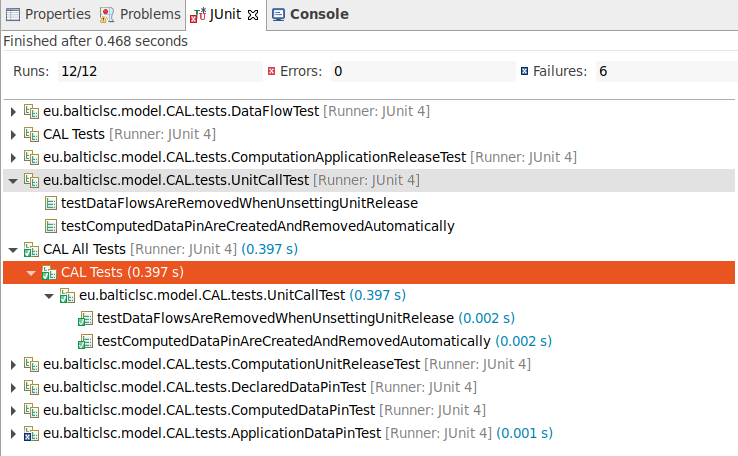
\includegraphics[width=0.90\linewidth]{./images/sirius-desktop-metamodel-tests.png}
	\caption{Wynik uruchomienia testów automatycznych
  metamodelu}\label{rys:sirius-desktop-metamodel-tests}
\end{figure}
% \end{noindent}

W przypadku tego metamodelu są przygotowane
jedynie dwa testy, więc nie było potrzeby dzielić je na grupy
(\emph{\selectlanguage{english}test suites}) --- jest tylko
jedna grupa nadrzędna \emph{\selectlanguage{english}CAL All Tests}, która
zawiera w sobie grupę
\emph{\selectlanguage{english}CAL Tests}, która zawiera poszczególne testy.
